\subsection{Vector Timing Correlation}
\label{sec:VTC}
\begin{figure}[t]
	\centering
	\vspace{-15pt}
	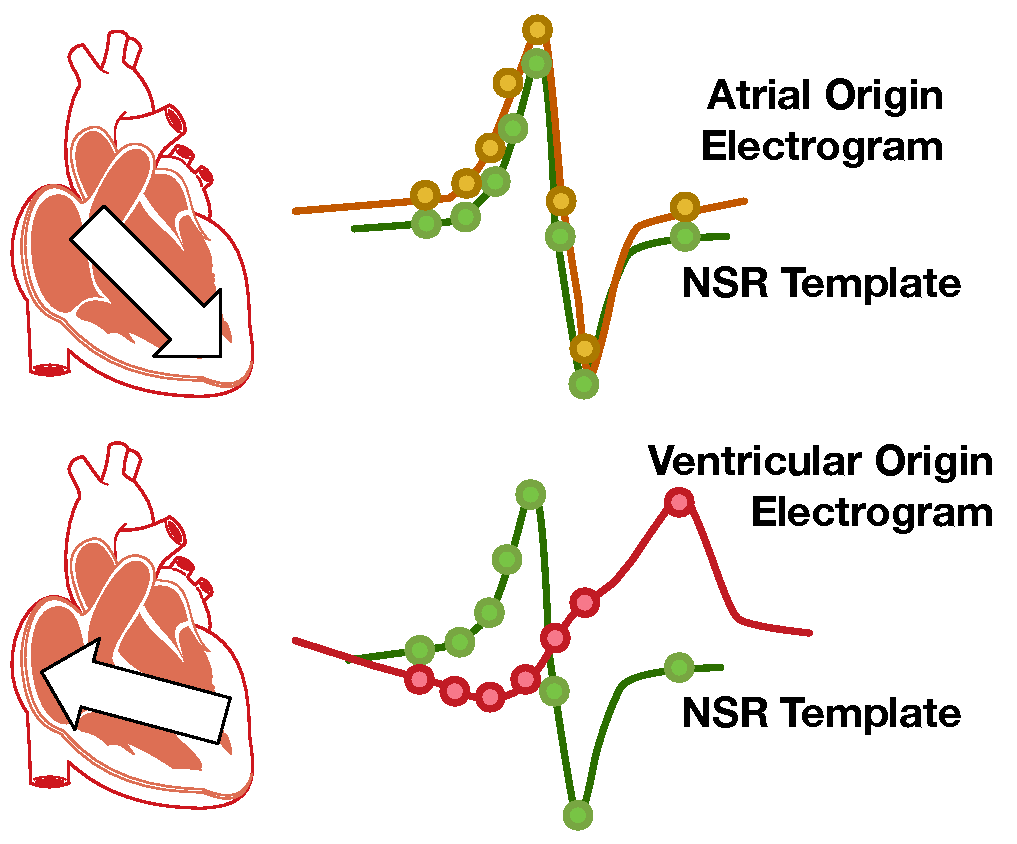
\includegraphics[scale=0.3]{figures/VTCEGMCompare}
	\caption{\small \acp{EGM} of different origin have different morphologies. The correlation of an \ac{EGM} with respect to a stored \ac{EGM} template is used to determine the origin.}
	\label{fig:egmmorphology}
	\vspace{-10pt}
\end{figure}
%\caption{\small \acp{EGM} of different origin have different morphologies, while \acp{EGM} of same origin have very similar morphologies.}
It has been clinically observed that a depolarization wave originating in the ventricles (as produced during \ac{VT} for example) will in general produce a different \ac{EGM} morphology than a wave originating in the atria (as produced during \ac{SVT}) \cite{compass}.
See Fig. \ref{fig:egmmorphology}.
%
A morphology discriminator measures the correlation between the morphology of the current \ac{EGM} and that of a stored \emph{template} \ac{EGM} acquired during normal sinus rhythm.
If the correlation is above a pre-set threshold for a minimum number of beats, then this is an indication that the current arrhythmia is supraventricular in origin.
Otherwise, it might be of ventricular origin.

Boston Scientific's implementation of a morphology discriminator is called Vector and Timing Correlation (VTC).
VTC first samples 8 \emph{fiducial} points $\egm_i,i=1,\ldots,8$ on the current \ac{EGM} $\egm$ at pre-defined time instants.
Let $\egm_{m,i}$ be the corresponding points on the template \ac{EGM}.
The correlation is then calculated as \cite{compass}
$\rho_{new} = \frac{(8\sum \egm_i \egm_{m,i} - (\sum \egm_i)(\sum \egm_{m,i}))^2}{(8\sum \egm_i^2 - (\sum \egm_i)^2)(8\sum \egm_{m,i}^2 - (\sum \egm_{m,i})^2)}    $
Note that $\egm_m$ is a constant for the purposes of this calculation: it does not change during an execution of VTC. 
If 3 out of the last 10 calculated correlation values exceed the threshold, then \ac{SVT} is decided and therapy is withheld.

The system of Fig. \ref{fig:HVTC} implements the VTC discriminator.
As before, $t$ is a local clock.
$\mu$ accumulates the values of the current \ac{EGM}, $\alpha$ accumulates the product $\egm_i \egm_{m_i}$, 
$\beta$ accumulates $\egm_i^2$.
State $w$ is an auxiliary state we need to establish the STORMED property.
$\vec{\nu}$ is a 10D binary vector: $\vec{\nu}(i) = -1$ if the $i^{th}$ correlation value fell below the threshold, and is $+1$ otherwise.
$L_3$ is the state of $\Sys_{TCFI}$: the guard condition $L_3 \leq th$ indicates that all its entries have values less than the tachycardia threshold, which is when $\Sys_{VTC}$ starts computing.
$BeatEnds$ indicates the `end' of an \ac{EGM}, measured as a window around the peak sensed by $\Sys_{Sense}$.  
%
\begin{figure}[t]
\centering
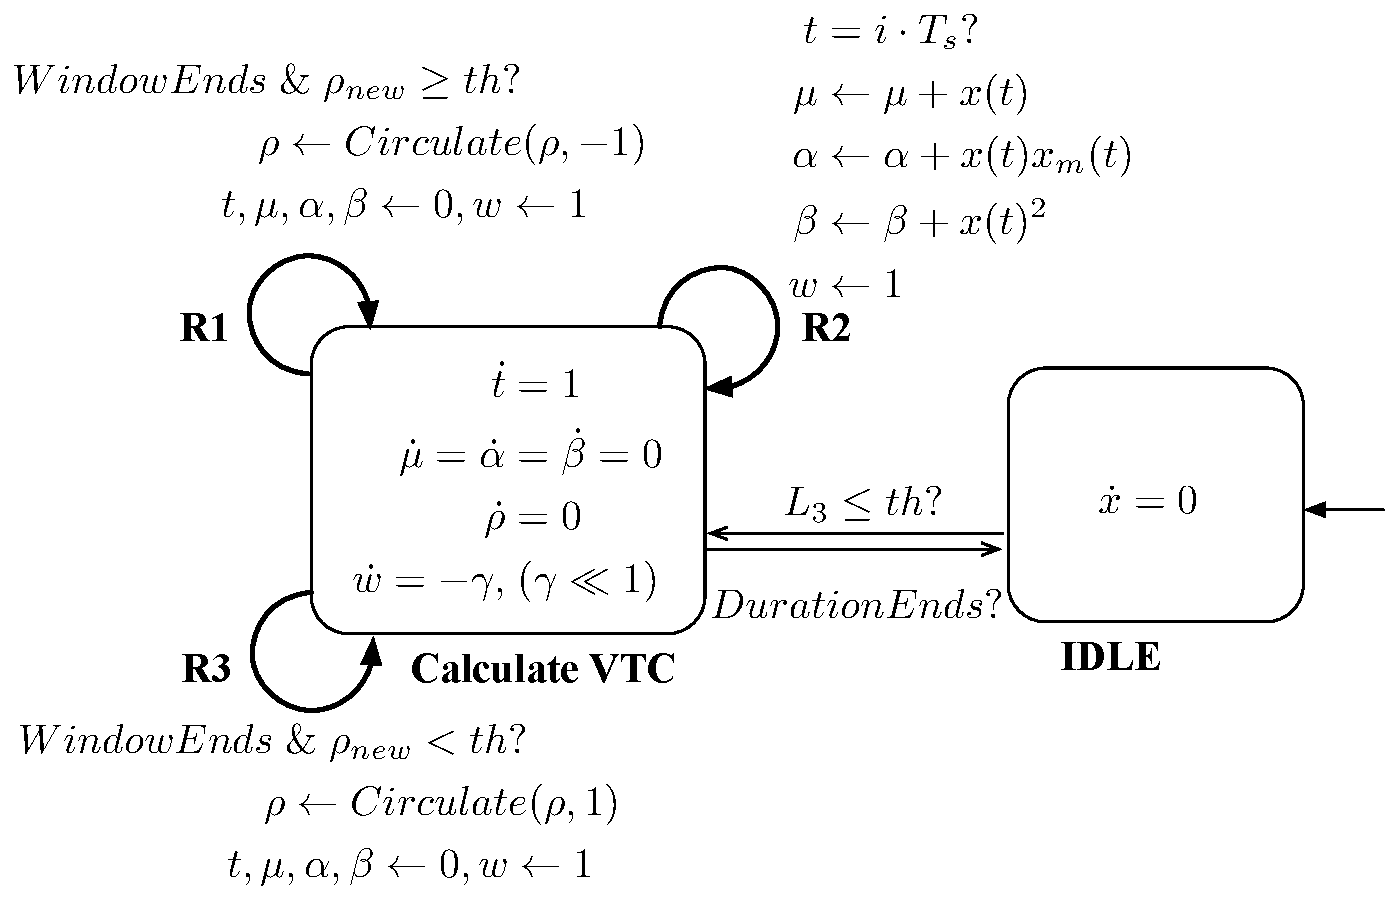
\includegraphics[scale=0.325]{figures/VTC1v2}
\vspace{-10pt}
\caption{VTC calculation. $iT_s$ is the sampling time.}
\vspace{-10pt}
\label{fig:HVTC}
\end{figure}
%
\begin{lemma}
	\label{lemma:vtc}
	$\Sys_{VTC}$ is STORMED.
	\end{lemma}
\begin{prf}
\textbf{S}eparability obtains by observing that a uniform minimum time passes between beats and between samples. 
\textbf{T}ISG is immediate.
\textbf{O}-minimality is established by observing that all sets and functions are definable in $\Lc_{\exp}$. \textbf{ED} holds because the state space is bounded.
We now show monotonicity.
The state of the system is $x = (t , \mu ,\alpha, \beta , \vec{\nu}, w)^T \in \Re^{4+10+1}$
Let $\phi = (\phi_c,\phi_\mu,\phi_\alpha,\phi_\beta,\phi_1,\ldots,\phi_{10},\phi_w)^T \in \Re^{15}$ be the corresponding vector.
For flows in mode CalculateVTC, we seek a $\phi$ and $\varepsilon > 0$ such that 
$\phi \cdot (t+\tau -  t , \mathbf{0} , -\gamma(t+\tau) + \gamma t) = \phi_c \tau + \phi_w(-\gamma \tau) \geq \varepsilon \sqrt{\tau^2 + \gamma^2\tau^2}$,
which is equivalent to 
$\boxed{\phi_c - \phi_w\gamma \geq \varepsilon \sqrt{1 + \gamma^2}}$.
Reset monotonicity provides three more constraints on $\phi$ and $\varepsilon$:
\begin{eqnarray*}
&\mathbf{(R1)} &
\phi \cdot (-t, -\mu , -\alpha , -\beta ,\nu_2 - \nu_1 , \nu_3 - \nu_2 , \ldots , -1 - \nu_{10})
\\	
&=& -\phi_c t -\phi_\mu \mu -\phi_\alpha \alpha - \phi_\beta \beta + \sum_{i=1}^{10}\phi_i(\nu_{i+1}-\nu_i) 
\\
&&+ \phi_w(1-w) \stackrel{Want}{\geq} \zeta
%
%
\\
%
%
&\mathbf{(R2)} &
\phi \cdot (t-t , \egm , \egm\cdot \egm_m, \egm^2 , \mathbf{0} , 1-w)
\\
&=& \phi_\mu \egm + \phi_\alpha \egm \egm_m+ \phi_\beta \egm^2 + \phi_w (1-w) \stackrel{Want}{\geq} \zeta > 0
%
%
\\ 
 %
 %
\\ &\mathbf{(R3)} &
 -\phi_c t -\phi_\mu \mu -\phi_\alpha \alpha - \phi_\beta \beta + \sum_{i=1}^{10}\phi_i (\nu_{i+1}-\nu_i) 
 \\
 && + \phi_w(1-w) \stackrel{Want}{\geq} \zeta
\end{eqnarray*}
where $\nu_{11} \defeq -1$ in $\mathbf{R1}$ and $\nu_{11}\defeq 1$ in $\mathbf{R3}$.
%
Combine $\mathbf{R1}$ and $\mathbf{R3}$ by choosing $\phi_1 = \ldots = \phi_{10}=\phi_\mu = \phi_\alpha = \phi_\beta = 0$:
\begin{eqnarray*}
\label{eq:R23}
\mathbf{(R1,3)}\; -\phi_c t + \phi_w(1-w) \geq \zeta
\\
\mathbf{(R2)}\; \phi_w(1-w) \geq \zeta
\end{eqnarray*}
Now note that when a reset occurs, $0<w \leq 1-\gamma T_s \defeq w_m$ where $T_s$ is the smallest sampling period, and that $t\leq 10B$, $B$ = the maximum peak-to-peak interval, so $\mathbf{(R2)} ,\mathbf{(R1,3)} $ can be jointly satisfied if $\boxed{-\phi_c10B + \phi_w(1-w_m) \geq \zeta}$.
The 2 boxed equations can be jointly satisfied.
	\end{prf}